%%%%%%%%%%%%%%%%%%%%%%%%%%%%%%%%%%%%%%%%%%%%%%%%%%%%%%%%%%%%%%%%%%%%%%%%%%%%%%%%%%%%%%%%%%%%%
%%									Chapitre 1											%
%%%%%%%%%%%%%%%%%%%%%%%%%%%%%%%%%%%%%%%%%%%%%%%%%%%%%%%%%%%%%%%%%%%%%%%%%%%%%%%%%%%%%%%%%%%%%
\chapter{Introduction}\label{chap:intro}
	\citationChap{
	The thing about quotes on the internet is that you can not confirm their validity
	}{Abraham Lincoln}
	\minitoc
	\newpage

%%%%%%%%%%%%%%%%%%%%%%%%%%%%%%%%%%%%%%%%%%%%%%%%%%%%%%%%%%%%%%%%%%%%%%%%%%%%%%%%%%%%%%%%%%%%%



% Début du chapitre

\section{Context of the Thesis}\label{sec:intro.context}
	\subsection{What do we study and why?}\label{sec:intro.context.what}
	    \gls{mab}

	\subsection{Regret minimization}\label{sec:intro.context.regret}
	\gls{regret minimization}
	
	On va ici placer des éléments graphiques (voir tableau~\ref{tab:exemple} et figure~\ref{fig:exemple}), juste pour avoir des entrées dans les listes des figures et des tableaux. On remarquera l'utilisation des sous-figures~\ref{sub:Antibes} et~\ref{sub:SaintJeannet}.

	\begin{tableth}
		\caption[Légende courte pour l'exemple de tableau]{Un tableau avec une légende tellement longue que ce serait hideux dans la liste des tableaux}
			\label{tab:exemple}
		\begin{tabular}{c|c}
			Coucou	& Au revoir\\
			\hline
			maman	& papa
		\end{tabular}
	\end{tableth}

	\begin{figureth}
		\begin{subfigureth}{0.4\textwidth}
			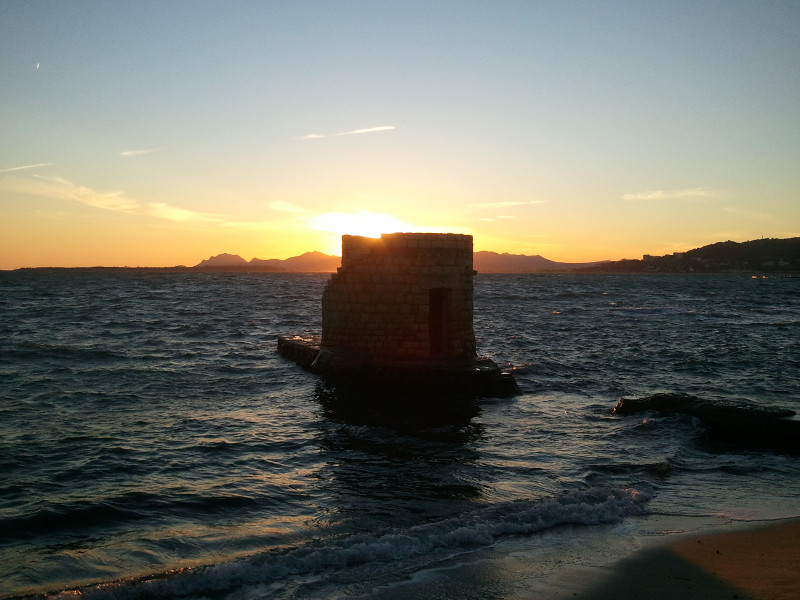
\includegraphics[width=\linewidth]{Chapter1/img/Antibes}
			\caption{Photo du Cap d'Antibes}
				\label{sub:Antibes}
		\end{subfigureth}
		\begin{subfigureth}{0.4\textwidth}
			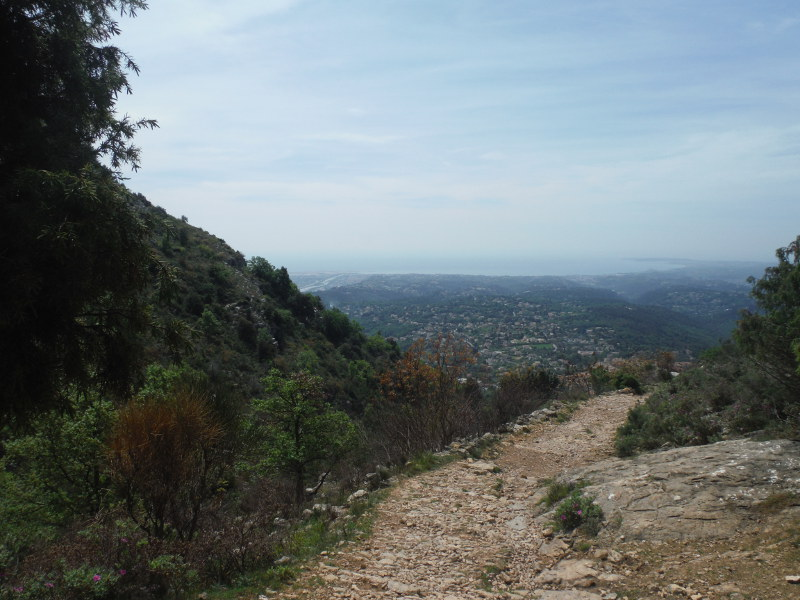
\includegraphics[width=\linewidth]{Chapter1/img/SaintJeannet}
			\caption{Saint Jeannet, depuis son Baou}
				\label{sub:SaintJeannet}
		\end{subfigureth}
		\caption[Légende courte pour la figure]{Exemple d'utilisation des sous-figures. J'utilise ici volontairement une légende longue.}
			\label{fig:exemple}
	\end{figureth}

	\subsection{Pure exploration}\label{sec:intro.context.pure}
	\gls{bai}
	
	Rien de spécial à propos des math, hormis l'illustration des symboles listés en fin de document, tels \gls{alpha} ou \gls{gamma}, qui peuvent être utilisés indifféremment en mode \emph{in-line} ou dans des équations\footnote{Le lecteur notera que \texttt{hyperref} ajoute un lien cliquable sur chaque entrée des différents glossaires.} :
	\begin{equation}
		\gls{alpha}=\nicefrac{\gls{gamma}}{2}
		\label{eq:alphagamma}
	\end{equation}
Les entrées des glossaires peuvent même être appelés dans des figures (PDF avec surcouche \LaTeX, ou Ti\textit{k}Z).

\section{Pure Exploration}\label{sec:intro.pe}
    
\section{Black-Box Optimization and Bandits with Many Arms}\label{sec:intro.black}
    \subsection{Infinite-armed bandits}\label{sec:intro.black.infinite}
    
    \subsection{Continuum-armed bandits}\label{sec:intro.black.continuum}
    
\section{Applications}\label{sec:intro.application}
    \subsection{Hyper-parameter optimization}\label{intro.application.hpo}
    \gls{hpo}
    
    \subsection{Other applications}\label{intro.application.other}
    
\section{A Brief Summary of the Contributions}\label{sec:intro.contributions}

\paragraph{List of published/peer-reviewed papers}

\cite{shang2020t3c,shang2018adaptive,shang2019dttts,shang2019adaptive,degenne2020game,shang2020vector}.

\paragraph{List of unpublished papers/preprints}

\section{Organization of the Thesis}\label{sec:intro.organization}

\newpage
\bibliographystyle{plain}
\bibliography{library}
